\chapter{Metodologia}
\label{cap:03}

Descrever metodologia, materiais e métodos utilizados no estudo, bem como os procedimentos experimentais realizados, nesta etapa será descrito vários assuntos sobre os passos a serem realizados iniciando com o levantamento dos dados, para uma analise e estudo posteriormente analisando todos os processos que são realizados, afim de iniciar o desenvolvimento.


\begin{figure}[ht]
    \caption{Passos feito na plataforma miro}
    \centering
    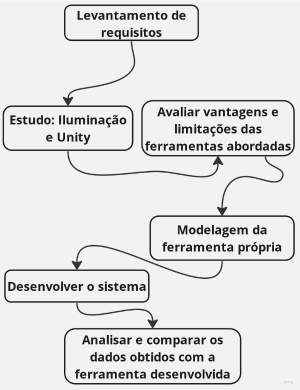
\includegraphics{imagens/Diagrama.jpg}

    Fonte: Feito pelo autor
    \label{fig:diagrama}
\end{figure}

\section{Levantamento de Requisitos}

Nessa sessão será abordado a pesquisa qualitativa feita a partir da ferramenta \textit{Relight} que usa de um algoritmo para identificação de camadas em uma imagem, assim, quando a imagem é colocada na ferramenta ela faz um mapeamento das áreas altas e baixas para criar as camadas, por esse motivo as camadas que são denominadas como mais alta recebe mais luz do que as mais baixas.

Porém a ferramenta tem uma funcionalidade a mais onde é possivel definir em que nível está a luz, fazendo com que a iluminação do objeto possa vir das camadas mais a baixo para as camadas acima, está ferramenta com a luz funciona como um pincel de adicionar em softwares de pintura, pois ela recebe a luz já existente na foto e complementa por cima com a luz própria, podendo ser de qualquer cor.

A seguir será mostrado na tabela, onde terá a avaliação qualitativa referente a vários tipos de imagens testadas a partir da ferramenta, que para efeitos deste trabalho serão utilizados os valores de alta resolução como acima de 720 pixels, média resolução entre 720 e 256 pixels e baixa resolução abaixo de 256 pixels, retratado na tabela:

Avaliação qualitativa da ferramenta

\begin{tabular}{l r r r}
    Imagem    & Alta Resolução & Média Resolução & Baixa Resolução \\
    Objetos   & Funciona       & Funciona        & Restrição       \\
    Humanos   & Funciona       & Funciona        & Restrição       \\
    Paisagens & Funciona       & Problema        & Problema        \\
\end{tabular}

Nessa tabela, foi adotado três categorias para descrever o funcionamento: Funciona, Restrição e Problema.
A primeira categoria é utilizada para descrever que a imagem utiliza se comportou de forma correta, Restrição é a categorização para as imagens que funcionam mas em alguns casos ou áreas da imagem geram problemas, já a categoria Problema indica os casos onde a luz não reconhecia as formas de maneira correta.

\section{Estudo: Python e suas bibliotecas}
Nesta seção, será abordado sobre as diferentes bibliotecas estudadas para que a análise pudesse ser feita com o melhor aproveitamento da linguagem.
será mostrado também alguns tópicos referente ao estudo do python como linguagem em geral.

Para iniciar o estudo das bibliotecas antes, deve se entender melhor sobre os ambientes do python como o ambiente virtual, além de estudar como é o funcionamento das IDEs com o ambiente python dá mesma forma.


\subsection{PyTorch}

Para o uso da SegmentAnything o pyTorch é uma das dependencias cruciais, já que ele aborda todo o processamento usado por placas de video e sistemas integrados com maior facilidaade. 
O estudo dessa biblioteca se faz necessário apenas para a instalação de seus softwares dependentes como o uso do NVIDIA CUDA entre outros sistemas terceiros para o funcionamento do Segment Anything.

\subsection{Scikit-image}

O Scikit será extremamente necessário para a análise dos recursos e resultados obtidos, pois é com ele que conseguimos facilmente gerar as estatísticas como o MSE por exemplo.
Não apenas isso mas o estudo dessa ferramneta deve vir analóga ao estudo dos métodos de estimativa comparando duas imagens.

\subsection{OpenCV}

O OpenCV (\texttt{cv2}) será empregado para lidar com tarefas relacionadas ao processamento de imagens, como leitura, conversão e redimensionamento.
Ele será utilizado para ler as imagens a partir do disco (\texttt{cv2.imread}) e convertê-las entre diferentes espaços de cores para garantir a consistência de dados durante o processamento. Por exemplo, a função \texttt{cv2.cvtColor} será usada para converter as imagens do formato BGR para RGB, alinhando-as ao formato de cores esperado pelo modelo de segmentação. Além disso, o OpenCV será usado para redimensionar as imagens (\texttt{cv2.resize}) a fim de assegurar que elas possuam o mesmo tamanho antes de realizar comparações e cálculos de correlação. Um dos métodos-chave será o cálculo da Correlação Cruzada Normalizada (NCC), que será realizado por meio da função \texttt{cv2.matchTemplate}. Esse método permitirá medir a similaridade entre a imagem segmentada e a imagem esperada, fornecendo uma métrica quantitativa para avaliar a precisão do processo de segmentação.

\subsection{Numpy}
No projeto, o \texttt{numpy} será fundamental para a manipulação eficiente de arrays multidimensionais, que representarão as imagens processadas. O \texttt{numpy} será utilizado para criar e gerenciar esses arrays, facilitando a realização de operações matemáticas e comparações pixel a pixel nas imagens. Por exemplo, a função \texttt{np.zeros} será utilizada para inicializar uma matriz de zeros que servirá como base para a imagem segmentada final na função de geração de máscara. Além disso, o \texttt{numpy} permitirá a execução de operações eficientes, como a comparação entre arrays de imagens para verificar a igualdade de pixels com a função \texttt{np.array\_equal}. As imagens serão normalizadas convertendo os valores de pixel para um formato de ponto flutuante, possibilitando uma análise mais precisa ao dividir os valores por 255.0.

\section{Estudo: Inteligência Artificial}
Nesse estudo será demonstrado algumas das partes que serão necessárias para a criação da análise posteriormente, 
inicialmente foi preciso uma serie de estudos sobre todas as possibilidades relacionadas as possíveis segmentações realizadas, 
a seguir cada tipo de segmentação será melhor explicada.

\subsection{Segmentação por mascára}
A segmentação por máscara utiliza um modelo para identificar e isolar regiões específicas dentro de uma imagem. 
O modelo gera uma máscara binária onde a região segmentada é representada por 1 e o fundo por 0.
 Este método é eficaz para separar objetos ou áreas de interesse em imagens, permitindo uma análise mais detalhada dessas regiões específicas.

\subsection{Segmentação por pontos de clique}
Neste método, o usuário seleciona pontos dentro da área que deseja segmentar.
É utilizo esses pontos como referências para definir os limites da região de interesse.
 A segmentação é então ajustada com base na localização desses pontos, oferecendo um controle mais preciso sobre as regiões segmentadas, especialmente em imagens complexas.

\subsection{Segmentação por caixa de delimitação}
Aqui, o usuário fornece uma caixa delimitadora ao redor do objeto ou área de interesse. 
O modelo então realiza a segmentação dentro dessa caixa. 
Esse método é útil para rapidamente identificar e segmentar objetos que podem ser facilmente contidos dentro de uma área retangular, facilitando a definição da região de interesse.


\subsection{Segmentação por texto}
A segmentação por texto permite ao usuário descrever a região ou objeto desejado em termos textuais. 
O modelo utiliza essa descrição para identificar e segmentar a área correspondente na imagem. 
Este método é útil quando a descrição do objeto é mais clara em palavras do que em detalhes visuais, oferecendo uma maneira eficiente de segmentar com base em descrições contextuais.


\subsection{Segmentação interativa}
Este método combina várias abordagens interativas, como pontos de clique e caixas de delimitação, permitindo que o usuário refine a segmentação com base no feedback contínuo. 
A segmentação inicial pode ser ajustada e melhorada conforme o usuário fornece mais informações ou faz ajustes na área segmentada, resultando em uma segmentação mais precisa e adaptada às necessidades específicas.


\subsection{Segmentação automática}
Na segmentação automática, é aplicado algoritmos de segmentação sem intervenção do usuário. 
O modelo usa padrões aprendidos para identificar e segmentar automaticamente os objetos de interesse na imagem. 
Esse método é ideal para processar grandes volumes de dados ou quando a segmentação precisa ser realizada de forma rápida e eficiente em cenários bem definidos.

\section{Procedimentos e Técnicas}

Para o desenvolvimento desta pesquisa, foram realizados testes preliminares explorando toda a capacidade do modelo Segment Anything (SAM), com o intuito de validar a eficácia dos processos envolvidos na análise de segmentação de imagens. Durante essa fase inicial, foi constatado que o tempo de processamento se mostrou elevado, mesmo em um sistema com hardware moderno. Como resultado, optou-se por não utilizar a tecnologia NVIDIA CUDA, uma vez que o uso intensivo de processamento pela GPU não seria imprescindível para o escopo do projeto.

Com essa decisão tomada, iniciou-se uma nova bateria de testes envolvendo diferentes tipos de imagens, abrangendo diversas categorias visuais, a fim de avaliar o potencial de segmentação do SAM em variados contextos. Os resultados foram, em sua maioria, satisfatórios, com o modelo demonstrando desempenho adequado na maioria dos casos analisados.

Posteriormente, iniciou-se o desenvolvimento de imagens específicas, criadas pelo autor em estilo pixel art, para validar a performance do modelo em situações de segmentação por cor. Essa etapa exigiu ajustes no código, especialmente no que diz respeito à manipulação das camadas e formatos das imagens, além da tipagem adequada em Python. Esse processo envolveu pesquisas extensivas e múltiplas tentativas até a obtenção de um resultado satisfatório na geração de grupos de cores a partir das imagens.

Com o sistema de segmentação de imagens em funcionamento, iniciou-se a etapa de criação manual das camadas de segmentação. O autor definiu como deveriam ser os resultados esperados da segmentação proposta pela IA, segmentando um conjunto de 50 imagens em estilo pixel art com base em cores específicas para realizar as análises. A partir desse ponto, foi possível aplicar métodos existentes para a comparação entre duas imagens.

Inicialmente, foi desenvolvido um método próprio, denominado pelo autor como "Método de Espalhamento". Esse método parte do canto da imagem e realiza uma varredura pixel a pixel ao redor de cada ponto analisado, comparando diretamente com o resultado esperado. Caso a cor do pixel na imagem gerada seja diferente da cor prevista no resultado esperado, era gerada uma pontuação negativa. Se as cores coincidissem, o método prosseguia, continuando a busca por outras colorações na imagem base.


Sempre que vemos uma cor clara e logo depois uma escura, isso significa que há um relevo muito grande ali, por exemplo  na Figura \ref{fig:batman}

\begin{figure}[ht]
    \caption{História em quadrinhos, Batman}
    \centering
    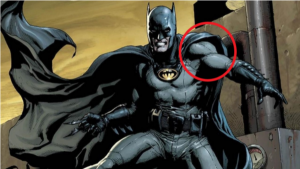
\includegraphics{imagens/batman.png}

    Fonte: \cite{Bazela2022-yg}
    \label{fig:batman}
\end{figure}

Nesse quadrinho do Batman, podemos ver que em seu ombro está muito claro e logo acima onde sua capa está vem uma cor muito escura, isso nos mostra que a profundidade da capa é grande, ao ponto de não chegar nenhuma luz até ela, é claro que precisamos levar em consideração que nas HQ’s em geral os contrastes são muito maiores, porque traz esse volume nos trajes. 

Partindo para o ramo da \textit{Unity} será preciso um aprendizado todo relacionado a iluminação dentro da ferramenta, uso dos objetos em cena e manipulação deles, pois para o desenvolvimento será necessário a criação de uma malha que forme a imagem, um sistema de camadas para que possa estabelecer profundidade, um sistema de alteração e manipulação da posição, cor e luminosidade do ponto de luz. E por fim um estudo básico de toda interface da \textit{Unity}.

Outro ponto importante no estudo, será a linguagem de programação \texttt{C\#} que é usada como alicerce para qualquer código que precise ser estruturado lá dentro, desde instanciar objetos dentro da cena até modificar configurações de câmera como movimento, posicionamento e angulo até para recebimento dos arquivos

\section{Avaliar vantagens e limitações das ferramentas abordadas}

O \textit{Relight} é uma ferramenta muito boa para processos de iluminação tanto para cenários como personagens, com uma boa modificação como profundidade, posição, cor e luminosidade, dando para o usuário a liberdade de dar personalidade as suas imagens.

Mas ainda existe várias limitações e elas que serão retratadas nessa seção, como foi visto na analise a cima na tabela é possível notar que quanto menor a imagem é, menos funcional ela passa a ser, por exemplo imagens em baixa resolução ou pixeladas começam a ter muitos problemas pois a luz não consegue distinguir os objetos na cena e muito menos paisagens pois com tantas cores perto uma das outras transforma a cena em uma desordem visual.

Além da ferramenta abordada acima existe também algumas outras opções no mercado para este tipo de processo, como o \textit{laigter} mas que ainda se envolve em uma limitação, que é o mapa de normais em apenas uma camada, o laigter atual na imagem fornecida pelo usuario como retratado na \ref{fig:laigter}.

\FloatBarrier
    \begin{figure}[ht]
        \caption{Imagens retiradas do github da ferramenta}
        \centering
        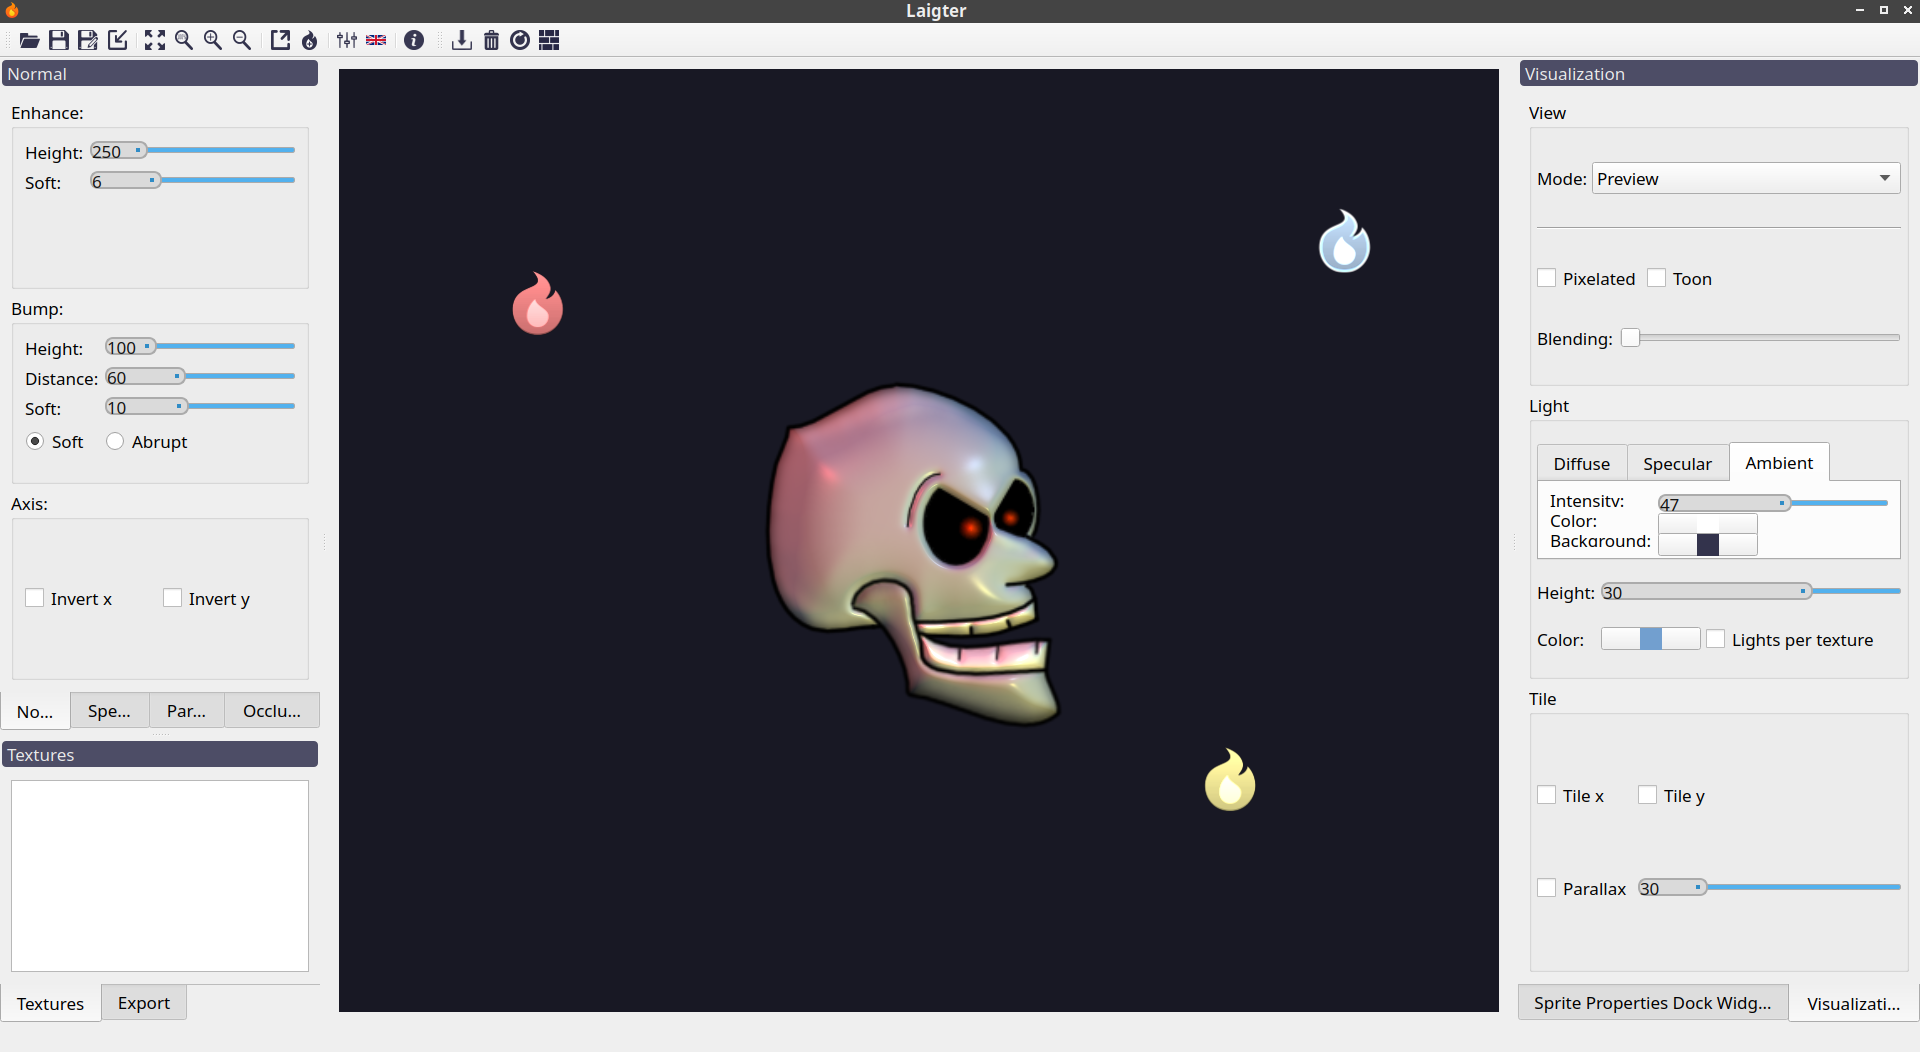
\includegraphics[scale=0.2]{imagens/laigter_example.png}
        \label{fig:laigter}
    \end{figure}
\FloatBarrier
    

\section{Modelagem da ferramenta}

Uma malha deverá ser criada por cima de toda a imagem e definir um inteiro para a profundidade, cada \textit{pixel} dá imagem deve receber uma profundidade como pode se observar na Figura \ref{fig:sketch}

\FloatBarrier
\begin{figure}[ht]
    \caption{Rascunho elaborado pelo autor}
    \centering
    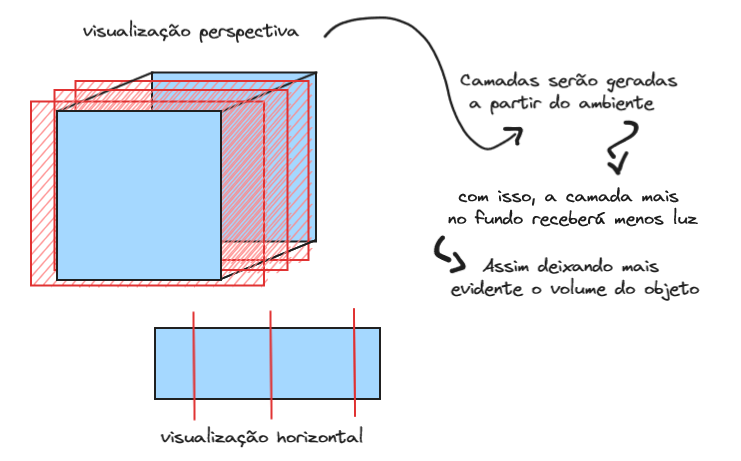
\includegraphics[scale=0.5]{imagens/Sketch.png}

    \label{fig:sketch}
\end{figure}
\FloatBarrier

Assim ele vai numerar toda a malha de \textit{pixels} na tela com números que podem ter uma variação maior dependendo do tamanho da imagem ( no caso de exemplo)

Será calculado de 1 a 9, mas com imagens imensas em alta resolução podemos pensar em usar de 1 a 100 ou até mais

Podemos pensar que dessa forma será possível utilizar essa profundidade para produzir uma luz pelas laterais ou pela frente e até atrás de elementos, sem perder sua funcionalidade até mesmo em imagens pequenas

Além disso, cada um desses valores definidos em cada \textit{pixel} da imagem, vão servir de referencia para criação de vários objetos, ele levará em consideração a distância e a variação de cor que foi atingida

Como por exemplo, se existir um objeto a frente da camada 1 até a 10 e um objeto atrás que está na camada 15, essa distancia de 5 camadas irá fazer o objeto dá frente se separar com o de trás transformando a cena com dois objetos ao invés de um


\section{Justificativa das Tecnologias a serem adotadas}

Será utilizado a IDE Visual Studio para a criação dos códigos que serão importados na \textit{Unity}, foi optado ele pois é o sistema mais robusto para a utilização do \texttt{C\#}.

Para o processo de desenvolvimento efetivo, além da IDE será usado a \textit{game engine}, Unity, que foi escolhida pela simplicidade em aplicar luz e criação de objetos bidimensionais em ambientes Tridimensionais, ou como é conhecido 2.5D, para assim poder criar com efetividade a malha e a luz aplicada a ela

\section{Avaliação Qualitativa}



\section{Objetivo da Metodologia}



\section{Design da Pesquisa}







\section{Amostragem}



\section{Procedimentos Analíticos}



\section{Critérios de Validação e Confiabilidade}



\section{Aspectos Éticos}



\section{Cronograma e Recursos}



\section{Limitações}

